\section{Introduktion}
Formålet med denne øvelse er at udarbejde en protokol stack til overførsel af filer via et RS-232 interface.
Systemet gør det muligt at overføre en fil fra en virtuel computer til en anden. Hvor den første virtuelle
maskine fungerer som client og den anden som server.
Clienten meddeler serveren hvilken fil der skal hentes, hvorefter serveren læser og sender denne, i pakker
af 1000 bytes af gangen. Clienten modtager så disse og gemmer dem i en fil.
Vi bruger i denne øvelse server og clienten fra øvelse 8. Forskellen fra øvelse 8 er at vi denne gang ikke
anvender socket-API til at udføre kald, i denne øvelse bruger vi kald til vores transportlag i en protocolstack som vi selv har udviklet. Brugerfladen er dog ens.

\section{Protokol}
De enkelte funktioner er delt op efter en lagdelt model, som kan ses på figur~\ref{fig:layers}.

\begin{figure}[h]
	\centering
	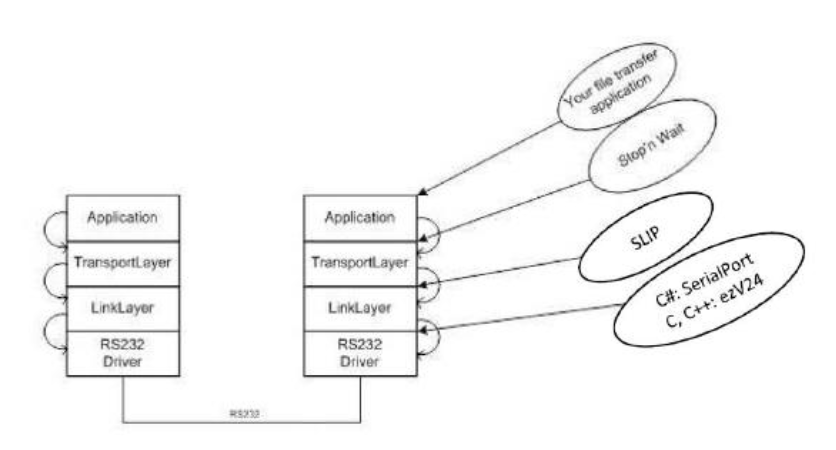
\includegraphics[width=0.7\linewidth]{figs/layers}
	\caption{}
	\label{fig:layers}
\end{figure}

\subsection{Application layer}
Vores applikationslag fungerer næsten på samme måde som i øvelse 8. Forskellen er dog at vi har udskiftet
TCP-kaldet med transportlags kald.

\subsection{Transport layer}
Transportlaget er implementeret via stop-and-wait protokol. Protokollen anvender en 16-bit checksum.
Se på figur~\ref{fig:segment} at laget overholder følgende segment:

\begin{figure}[h]
	\centering
	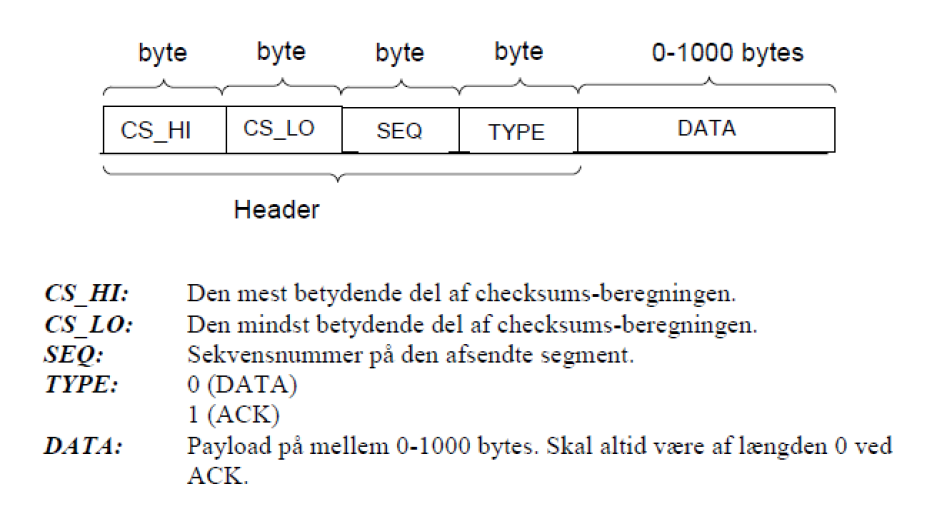
\includegraphics[width=0.7\linewidth]{figs/segment}
	\caption{}
	\label{fig:segment}
\end{figure}

Da vi fra transportlaget ønsker at sende et byte array videre til linklaget, som er større end det array vi
modtager fra applikationslaget, indeholder transportlag sit eget buffer array, som er ”HeaderSize” større
end applikations arrayet. Vi indsætter sekvens i tredje byte og type i fjerde byte. For god ordens skyld
initierer vi de to første bytes til 0, men disse bliver overskrevet når vi senere beregner vores checksum.
Derefter kopieres arrayet fra applikations laget ind i det nye array.
På baggrund af hele det nye array, altså også sekvens nummer og type, beregnes checksummen, og
indsættes på de første to pladser.
Til sidst sendes det nye array til link laget, og dette fortsættes indtil vi modtager en ack fra modtageren. Det
hele ses i funktionen herunder:

\begin{lstlisting}
public void send(byte[] buf, int size)
{
	buffer [0] = 0; //checksum high - replaces in calcChecksum
	buffer [1] = 0; //checksum low - replaces in calcChecksum
	buffer [2] = seqNo; //seq number
	buffer [3] = 0; //Type (0 = data / 1 = ack)
	Array.Copy(buf, 0, buffer, HEADER_SIZE, buf.Length);
	
	checksum.calcChecksum (ref buffer, size + HEADER_SIZE); //insert checksum
	
	bool ackReceived = false;
	
	do 
	{
		link.send (buffer, size + HEADER_SIZE);
		
		ackReceived = receiveAck ();
	} while (!ackReceived);
}
\end{lstlisting}

På modtager siden starter vi med at modtage arrayet fra modtageres link lag. Vi beregner om
checksummen stemmer med de overførte data, og sender en ack tilbage baseret på resultatet. Vi kopierer
derefter arrayet over i et mindre array for at fjerne headeren. Dette gentages hvis det modtagne data ikke
stemte overens med checksummen. Til sidst returneres hvor mange bytes der i alt blev modtaget, minus
headerens data som vist herunder:

\begin{lstlisting}
public int receive (ref byte[] buf)
{
	int receivedBytes = 0;
	bool receivedOk = false;
	
	do 
	{
		receivedBytes = link.receive (ref buffer);
		receivedOk = checksum.checkChecksum (buffer, receivedBytes);
		sendAck (receivedOk);
		Array.Copy(buffer, HEADER_SIZE, buf, 0, buf.Length);
	} while(!receivedOk);
	
	return receivedBytes - HEADER_SIZE;
}
\end{lstlisting}

For at teste om data bliver sendt igen i tilfælde af fejl, har vi lavet følgende test setup hvor der testes med
en false ack, samt fejl i checksum:

\begin{lstlisting}
//Test Program
int receivedBytes = link.receive (ref buf);
sendAck (false);
Console.WriteLine ("test - transport sent false ack");

receivedBytes = link.receive (ref buf);
buf [0] = 47;
sendAck( checksum.checkChecksum (buf, receivedBytes));
Console.WriteLine ("test - transport with wrong checksum - !ack sent");

receivedBytes = link.receive (ref buf);
sendAck( checksum.checkChecksum (buf, receivedBytes));
Console.WriteLine ("test - transport with ok checksum - ack sent");

return receivedBytes;
\end{lstlisting}

På denne måde får vi testet at vores protokol stack overholder 3 af de 4 scenarier fremsat af underviseren.
Det sidste scenarie lykkedes desværre ikke at få gennemført. Scenarierne ses på figur~\ref{fig:sekvensdia} på side~\pageref{fig:sekvensdia}, udleveret af
underviser:

\begin{figure}[h]
	\centering
	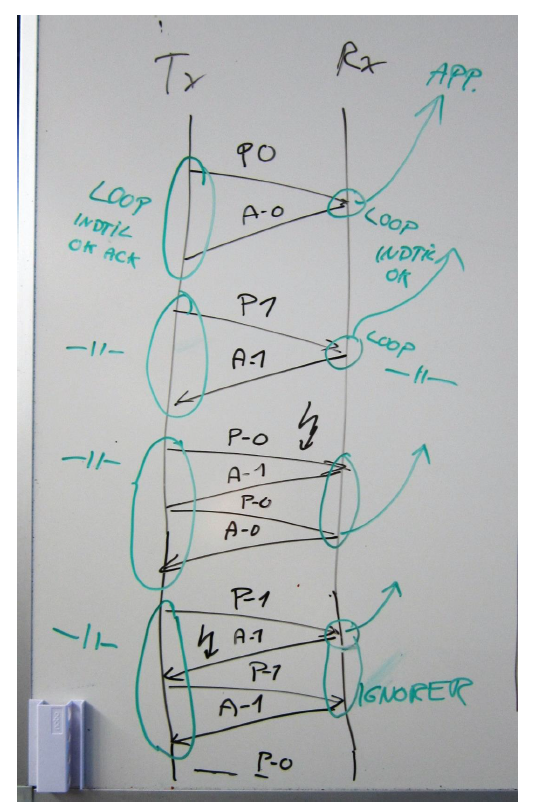
\includegraphics[width=0.7\linewidth]{figs/sekvensdia}
	\caption{}
	\label{fig:sekvensdia}
\end{figure}

\subsection{Link layer}
I denne øvelse skulle vi udvikle vores egen protokol med start og stop karakter ‘A’. Karakter ’A’ bliver derfor
erstattet med ’BC’ og ’B’ er erstattes med ’BD’ som vist herunder på figur~\ref{fig:bd}.

\begin{figure}[h]
	\centering
	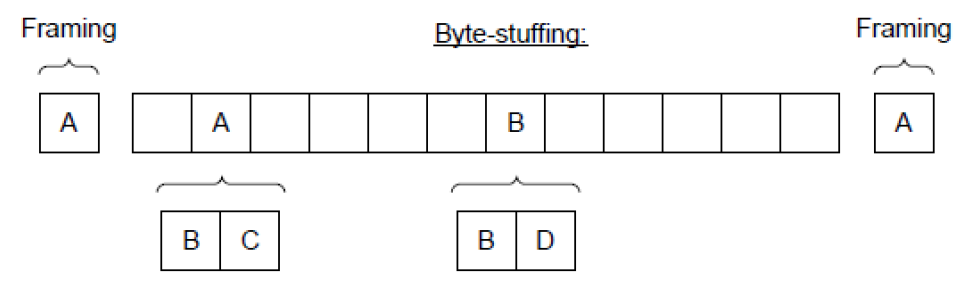
\includegraphics[width=0.7\linewidth]{figs/bd}
	\caption{}
	\label{fig:bd}
\end{figure}

Her er et eksempel på vores link lag. Her implementeres vores protokol i send funktionen.

\begin{lstlisting}
public void send (byte[] buf, int size)
{
	buffer[0] = 65; //Insert A at start
	int bytesToSendIndex = 1;
	for (int i = 0; i < size; i++) 
	{
		if (buf [i] == 65) 
		{
			buffer[bytesToSendIndex] = 66;
			bytesToSendIndex++;
			buffer[bytesToSendIndex] = 67;
			bytesToSendIndex++;
		}
		else if (buf [i] == 66) 
		{
			buffer[bytesToSendIndex] = 66;
			bytesToSendIndex++;
			buffer[bytesToSendIndex] = 68;
			bytesToSendIndex++;
		} 
		else 
		{
			buffer [bytesToSendIndex] = buf [i];
			bytesToSendIndex++;
		}
	}
	buffer [bytesToSendIndex] = 65;
	bytesToSendIndex++;
	serialPort.Write (buffer, 0, bytesToSendIndex);
}
\end{lstlisting}

\subsection{RD232 Driver}
Her opretter vi det fysiske lag, som I dette tilfælde er vores RS-232-port og vores null-modem.

\begin{lstlisting}
public Link (int BUFSIZE)
{
	// Create a new SerialPort object with default settings.
	serialPort = new SerialPort("/dev/ttyS1",115200,Parity.None,8,StopBits.One);
		
	if(!serialPort.IsOpen)
		serialPort.Open();

	buffer = new byte[(BUFSIZE*2)+2];
}
\end{lstlisting}

\subsection{Server}
På vores server opretter vi et nyt transportlag med den ønskede bufsize når den startes. Derefter kaldes
file_server() med dette transportlag hvorefter der ventes på at modtage en forespørgsel på serveren. Når
denne modtages tjekker vi om filen eksisterer, hvis denne findes sendes denne.

\begin{lstlisting}
private file_server (Transport transport)
{
	try
	{
		Console.WriteLine("Server started - Listening for client");
		
		//Get filename
		
		string fileToSend = transport.readText();
		
		Console.WriteLine("Client trying to retrieve file: " + fileToSend);
		
		long fileSize = LIB.check_File_Exists (fileToSend);
		
		if (fileSize != 0)
		{
			transport.sendText("File found");
			
			sendFile (fileToSend, fileSize, transport);
		} 
		else 
		{
			transport.sendText("File not found");
			Console.WriteLine ("404 - File not found");
		}
	}
	catch (Exception ex) 
	{
		Console.WriteLine (ex.Message);
	}
	finally
	{
		Console.WriteLine ("Exit");
	}
}
\end{lstlisting}

\subsection{Client}
På vores klient opretter vi et nyt transportlag med den ønskede bufsize når den startes. Herefter kaldes
file_client() med filnavnet på fil den ønskes hentes, samt hvilket transportlag der ønsker kommunikeres
over. En svar modtages om størrelsen på filen modtages og herefter begynder clienten at modtage og
gemme filen.

\begin{lstlisting}
private file_client(String[] args, Transport transportStream)
{
	try
	{
		Console.WriteLine ("Retrieving file");
		
		string fileToReceive = (args.Length > 0) ? args[0] : "billede.jpg";
		
		transportStream.sendText(fileToReceive);
		
		//Read confirmation that file exists
		
		if (transportStream.readText() == "File found") 
		{
			receiveFile (fileToReceive, transportStream);
		} 
		else 
		{
			Console.WriteLine ("404 - File not found");
		}
	}
	catch (Exception ex)
	{
		Console.WriteLine ("Generel exception occured");
		Console.WriteLine(ex.Message);
	}
	finally 
	{}
}
\end{lstlisting}

\subsection{Test}
Serveren startes og venter på client.

\begin{figure}[h]
	\centering
	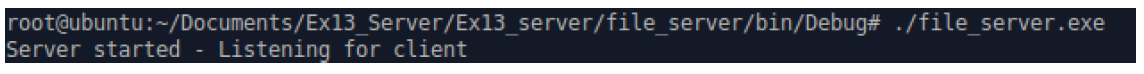
\includegraphics[width=0.7\linewidth]{figs/test1}
	\caption{}
	\label{fig:test1}
\end{figure}

Client sender hvilken fil der ønskes hentet.

\begin{figure}[h]
	\centering
	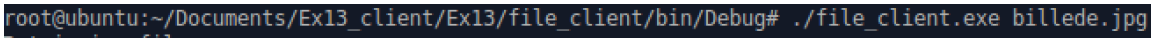
\includegraphics[width=0.7\linewidth]{figs/test2}
	\caption{}
	\label{fig:test2}
\end{figure}

Serveren modtager besked fra client og begynder at sende filen.

\begin{figure}[h]
	\centering
	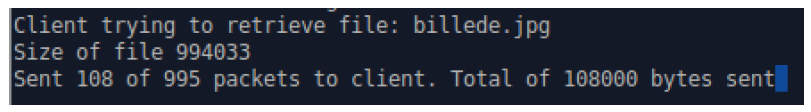
\includegraphics[width=0.7\linewidth]{figs/test3}
	\caption{}
	\label{fig:test3}
\end{figure}

Client begynder at modtage filen fra serveren.

\begin{figure}[h]
	\centering
	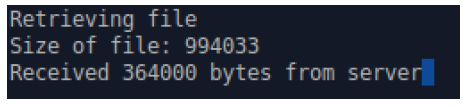
\includegraphics[width=0.7\linewidth]{figs/test4}
	\caption{}
	\label{fig:test4}
\end{figure}

\section{Konklusion}
Det praktiske forløb stemte overens med vores teori.